\section{Smartsensors}
\label{sec:approach}

Smartsensors make possible continuous mobile sensing by providing a
filter-based sensor API for application programming.  Applications create
{\em custom wake up conditions} for events of interest by choosing
from a pre-specified set of filtering algorithms and tuning their
parameters.  When these events occur, the main processor is woken up
and the application code is invoked. The result is that applications
view the sensors as ``smart'' sensors that generate relevant events
only.  This approach enables supporting a large number of sensing
applications while being significantly easier to program compared to
fully programmable offloading. Since the filters are pre-specified,
the device manufacturer can optimize their implementations for each
low-power processor, improving application portability between
devices.  Furthermore, it is possible to optimize the operation of
multiple applications that use common filters.

Figure~\ref{fig:smartarchitecture} shows the architecture of a
system that implements the Smartsensors abstraction.  Applications
interact with a sensor manager and define custom wake-up conditions by
choosing among the available pre-defined filters.  The figure also
shows that the architecture supports recognition libraries that
encapsulate the functionality of the Smartsensor to provide simple
wake up conditions for a large number of activities.  To keep the
complexity of filters low, our initial implementation limits filters
to operations on data collected from a single sensor.  Applications
that perform sensor fusion, are implemented by defining separate
independent wake up conditions on multiple sensors, and merging data on
the main processor.


\begin{figure}[t]
	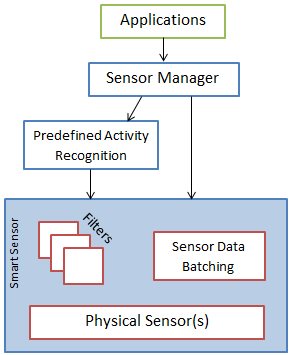
\includegraphics[width=3.1in]{android_smartsensor_architecture_proposed.png}
	\caption{Smartsensor system architecture.}
    \label{fig:smartarchitecture}
\end{figure}

The main challenge with our Smartsensors approach is defining the
appropriate set of event filters for each sensor.  First, there is a
trade-off between filter generality and accuracy.  Simple generic
filters can support a large set of applications, albeit no specific
application is likely to experience optimal performance.  Conversely, a
highly specialized filter may provide optimal performance but is only
applicable to a limited set of applications.  Second, there is also a
trade-off between filter complexity and power savings.  More complex
filters can reduce energy consumption by preventing unnecessary
wake-ups due to increase accuracy.  On the other hand, more complex
filters have higher computational demands, which require a larger and
hungrier peripheral processor.

Fortunately, continuous sensing applications are commonly structured
as modular pipelines of increasing selectivity and computational
complexity.  Early stages in the pipeline tend to be simpler but
execute with much higher frequency as only data that passes the
selection criteria is forwarded along to the next stage.
Moreover, while the application logic of different sensing application
varies widely, applications that use the same sensors tend to make use
of similar algorithms in the early stages of their event detection
pipelines.  We can thus determine potential filter candidates by
identifying these common algorithms.

For example, several accelerometer-based applications initially check
whether the acceleration magnitude exceeds a certain threshold in
order to determine if there is any movement. Also, the acceleration
data has significant noise, and hence many applications implement
low-pass filters to smoothen the accelerometer
readings~\cite{kangasFallDetection,libbyFootstepDetection}.  If
multiple accelerometer-based applications are running at the same
time, they are each checking for these events independently, possibly
resulting in redundant computation. Common steps such as thresholding
and low-pass filtering are excellent candidates for event filters.
Similarly, audio data is commonly passed though a high-cut or a
low-cut filter in order to reduce the amount of treble or bass in the
sound.  Image processing makes use of low-pass, high-pass and
band-pass filtering for noise reduction, and edge
detection~\cite{paul2005computer,marr1980theory}.


